\documentclass[a4paper,11pt]{article}
\usepackage[utf8]{inputenc}
\usepackage[T1]{fontenc}
\usepackage{amsmath, amssymb, amsfonts}
\usepackage{graphicx}
\usepackage{float}
\usepackage{booktabs}
\usepackage{geometry}
\usepackage{caption}
\usepackage{mathrsfs}  
\usepackage{subcaption}
\usepackage{siunitx}
\usepackage{hyperref}

\geometry{margin=2.5cm}
\graphicspath{{images/}}
\title{Continuum Mechanics for Cardiac Modelling}
\author{Diogo Amaro}
\date{\today}

\begin{document}
\maketitle

\section{Constitutive Modelling of Passive Myocardium}

The purpose of this section is to provide a mathematical description of the constitutive model used to characterize the mechanical behavior of the myocardium during passive diastolic filling. To this end, an overview of the fundamentals of soft tissue mechanics is presented, including the continuum mechanical framework, relevant kinematic and kinetic measures, and conservation laws. This is followed by a detailed discussion of hyperelastic modelling specific to cardiac tissue, including the role of fiber architecture and anisotropy.


\subsection{Continuum Mechanics}
Continuum mechanics is founded on the concept that a material (fluid, solid, or mixture) and its properties can be approximated by fields that are well defined almost everywhere~\cite{fung1977first, gurtin1982introduction, malvern1969introduction}. This continuum assumption considers the scale at which discrete microstructural variations appear to much smaller than the smallest scales of interest. This enables the averaging of material characteristics, transforming the discrete nature of materials into well-defined point-wise fields. Conservation laws can be derived to enable computational simulations of heart tissue, detailing its movement, deformation (kinematics), and stress responses (kinetics). This section briefly reviews these concepts.

\subsubsection{Kinematics of Large Deformation}
Kinematics is the study of motion of particles or objects and its subsequent deformation without reference to the cause, i.e., without explicit consideration of the masses and forces involved~\cite{bonet1997nonlinear}.  To describe the motion of a body in a \textit{d}-dimensional space, we define the region occupied by the body at $t=t_0$ as $\Omega_0 \subset \mathbb{R}^d$, to which we refer to as the \textit{reference configuration}. The choice of a reference configuration is completely arbitrary\footnote{More generally, any configuration that the body is capable of occupying (irrespective of whether it actually does or not) may serve as a reference configuration.}. Consequently, reference coordinates $\mathbf{X} \in \Omega_0$ describe the undeformed position of material particles within the body. In response to deformations, the material particles move to the coordinates $\mathbf{x} \in \Omega (t)$ at some time $t$, to which we refer to as the \textit{current configuration}.
Assuming that the reference coordinates, $\mathbf{X}$, and physical coordinates, $\mathbf{x}$, are related by a continuous displacement field $\mathbf{u}(\mathbf{X},t)$, i.e., $\mathbf{x}(\mathbf{X},t) = \mathbf{u}(\mathbf{X},t) + \mathbf{X}$, we can then define the Jacobian of the mapping relative to the reference configuration, also known as the deformation gradient tensor, as
\begin{equation}
\mathbf{F}=\frac{\partial \mathbf{x}}{\partial \mathbf{X}} = \nabla_\mathbf{X}\mathbf{u} + \mathbf{I},
\end{equation}
or, in Cartesian components, as
\begin{equation}
F_{ij}=\frac{\partial u_i}{\partial X_j}+\delta_{ij},
\end{equation}
where $\mathbf{I}$ is the identity tensor, with components described by the Kronecker delta symbol. 
\begin{equation}
\delta_{ij} =
    \begin{cases}
            1, &         \text{if } i=j,\\
            0, &         \text{if } i\neq j.
    \end{cases}
\end{equation}
For the description of local kinematics of any deformable body, we use the standard notation and convention
\begin{equation}
J=\det \mathbf{F}>0.
\end{equation}
Because $J$ quantifies the local change in volume, then for an incompressible material, the constraint 
\begin{equation}
J=\det \mathbf{F}\equiv 1
\end{equation}
must hold true. 

The concepts of displacement field and deformation gradient are introduced to quantify the change in shape of infinitesimal line elements in a solid body~\cite{bonet1997nonlinear}. To see this, let us draw a straight (red dashed) line on the undeformed configuration of a solid, as shown in Figure~\ref{fig:dx}.
\begin{figure}[H]
\centering
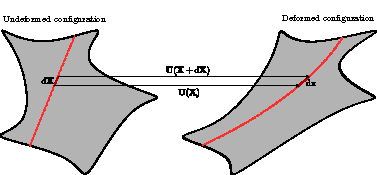
\includegraphics[width=0.75\textwidth]{images/dx.pdf}
\caption{Visualization of an infinitesimal line element in a deforming solid body. A reference straight line (dashed red) drawn on the undeformed configuration becomes a smooth curve upon deformation. However, a sufficiently small segment of this line, $\text{d}\mathbf{X}$, remains approximately straight after deformation, mapping to $\text{d}\mathbf{x}$ through the displacement field given by $\mathbf{u}(\mathbf{x}+\text{d}\mathbf{x})-\mathbf{u}(\mathbf{x})$. This shows that despite global curvature, local material behavior can be captured by stretch and rotation only.}
\label{fig:dx}
\end{figure}
The line would be mapped to a smooth curve on the deformed configuration. However, suppose we focus on a line segment $\text{d}\mathbf{X}$, much shorter than the radius of curvature of this curve, as shown in Fig.~\ref{fig:dx}.  The segment would be straight in the undeformed configuration, and would also be (almost) straight in the deformed configuration.  Thus, no matter how complex a deformation we impose on a solid, infinitesimal line segments are merely stretched and rotated by a deformation. We can then define the relation between infinitesimal line segments $\text{d}\mathbf{X}$ and $\text{d}\mathbf{x}$ as
\begin{equation}
\text{d}\mathbf{x}=\mathbf{F}\cdot \text{d}\mathbf{X}, \qquad \text{d}x_i=F_{ik}\cdot \text{d}X_k.
\end{equation}

Written out as a matrix equation, we have
\begin{equation}
\label{matdec}
\begin{bmatrix}
dx_1 \\
dx_2 \\
dx_3
\end{bmatrix}
=
\begin{bmatrix}
1 + \dfrac{\partial u_1}{\partial X_1} & \dfrac{\partial u_1}{\partial X_2} & \dfrac{\partial u_1}{\partial X_3} \\
\dfrac{\partial u_2}{\partial X_1} & 1 + \dfrac{\partial u_2}{\partial X_2} & \dfrac{\partial u_2}{\partial X_3} \\
\dfrac{\partial u_3}{\partial X_1} & \dfrac{\partial u_3}{\partial X_2} & 1 + \dfrac{\partial u_3}{\partial X_3}
\end{bmatrix}
\begin{bmatrix}
dX_1 \\
dX_2 \\
dX_3
\end{bmatrix}
\end{equation}

Following this logic, if a material fiber of initial length $l_0$ oriented along a unit vector $\mathbf{N}$ in the undeformed configuration, i.e. $\text{d}\mathbf{X}=l_0\mathbf{N}$, is stretched and rotated into a fiber of current length $l$ and orientation $\mathbf{n}$ in the deformed configuration, i.e. $\text{d}\mathbf{x}=l\mathbf{n}$, then we can quantify the squared length of infinitesimal fibers in the deformed configuration through the deformation tensors as  
\begin{equation}
||\text{d}\mathbf{x} ||^2 = \frac{l^2}{l_0^2} = \mathbf{N} \cdot \mathbf{C} \cdot \mathbf{N},
\end{equation}
\begin{equation}
||\text{d}\mathbf{X}||^2 = \frac{l_0^2}{l^2} = \mathbf{n} \cdot \mathbf{B^{-1}} \cdot \mathbf{n}.
\end{equation}

Here, $\mathbf{C}$ and $\mathbf{B}$ are the right and left Cauchy–Green deformation tensors, defined respectively as:

\begin{equation}
\mathbf{C} = \mathbf{F}^\mathrm{T}\cdot \mathbf{F}, \qquad C_{ij} = F_{ki}\cdot F_{kj},
\end{equation}
\begin{equation}
\mathbf{B} = \mathbf{F}\cdot  \mathbf{F}^\mathrm{T}, \qquad B_{ij} = F_{ik}\cdot F_{jk}.
\end{equation}

Both $\mathbf{C}$ and $\mathbf{B}$ are tensorial quantities used to model highly deformable solids such as the cardiac tissue and provide information about the local and directionally dependent stretch behavior of the material. Another commonly used kinematic quantity is the Green–Lagrange strain tensor, $\mathbf{E}$, that evaluates how much a given displacement differs locally from a rigid body displacement~\cite{zeidi2018mechanics}:
\begin{equation}
\mathbf{E} = \frac{1}{2}(\mathbf{C} - \mathbf{I}), \qquad E_{ij} = \frac{1}{2}(C_{ij} - \delta_{ij}).
\end{equation}
The development of a constitutive model requires coordinate independence and rigid body invariance ~\cite{ogden1997non, spencer2004continuum}. In order to account for those requirements, we define the principal invariants of $\mathbf{C}$ (and also of $\mathbf{B}$) as
\begin{equation}
\label{I123}
I_1=\text{trace}\,(\mathbf{C}), \qquad I_2=\frac{1}{2}[I_1^2-\text{trace}(\mathbf{C}^2)] \quad \text{and} \quad I_3=\det \mathbf{C},
\end{equation}
where $I_3=J^2=1$ for an incompressible material\footnote{The trace operator on $\mathbf{A} \in \mathbb{R}^{d\times d}$ is defined as trace ($\mathbf{A}$) $=\sum_i A_{ii}$}. These invariants, however, model isotropic materials. Because the cardiac tissue is anisotropic, additional pseudo-invariants must be defined for directional dependence~\cite{holzapfel2000continuum}. As previously mentioned, the myocardium exhibits its greatest stiffness along the fiber direction $\mathbf{f}$, meaning we can model anisotropy under the assumption the material has a preferred direction in the reference configuration, from now on denoted by the unit vector $\mathbf{f}_0$. Therefore, two additional invariants can be defined as
\begin{equation}
\label{I45}
I_4=\mathbf{f}_0\cdot(\mathbf{C}\mathbf{f}_0) \quad \text{and} \quad I_5=\mathbf{f}_0 \cdot(\mathbf{C}^2\mathbf{f}_0).
\end{equation}
Similarly, if there are two preferred directions, the second denoted by $\mathbf{s}_0$, then this introduces the invariants
\begin{equation}
\label{I67}
I_6=\mathbf{s}_0\cdot(\mathbf{C}\mathbf{s}_0) \quad \text{and} \quad I_7=\mathbf{s}_0 \cdot(\mathbf{C}^2\mathbf{s}_0).
\end{equation}
Associated with it and, additionally, a coupling invariant, denoted by $I_8$, defined by
\begin{equation}
\label{I8}
I_8=\mathbf{f}_0\cdot(\mathbf{C}\mathbf{s}_0)=\mathbf{s}_0\cdot(\mathbf{C}\mathbf{f}_0).
\end{equation}
Additionally, many models, including the one adopted in this work, consider splitting volumetric changes from distortional changes within the material. In this case, isochoric definitions of the deformation gradient are commonly used with corresponding changes to stretch tensors. In this case, we further decompose the deformation gradient $\mathbf{F}$ into volumetric ($\mathbf{F}_{\text{vol}}$) and isochoric ($\bar{\mathbf{F}}$) parts, as $\mathbf{F}=\bar{\mathbf{F}}\mathbf{F}_{\text{vol}}$ such that
\begin{equation}
\label{fdecomp}
\mathbf{F}_{\text{vol}}=J^{\frac{1}{3}}\mathbf{I} \quad \text{and} \quad \bar{\mathbf{F}}=J^{-\frac{1}{3}}\mathbf{F},
\end{equation}
leading to the definiton of the modified right Cauchy-Green tensor
\begin{equation}
\label{mrcgt}
\bar{\mathbf{C}}=\bar{\mathbf{F}}^\mathrm{T} \bar{\mathbf{F}}=J^{-\frac{2}{3}}\mathbf{C}.
\end{equation}
The reason for the decomposition of the deformation gradient $\mathbf{F}$ becomes clear once we introduce the constitutive law, particularly the strain energy function. Figure~\ref{fig:kinematics} provides a visual overview of the deformation mechanism of a solid body under the assumptions made throughout this Section.


\begin{figure}[H]
\centering
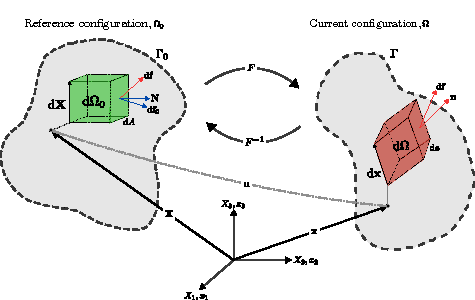
\includegraphics[width=0.75\textwidth]{images/kinematics.pdf}
\caption{General motion of a deformable body. The figure shows the mapping from a reference configuration $(\Omega_0, \Gamma_0)$, with material coordinates $\mathbf{X}_i$, to a deformed configuration $(\Omega, \Gamma)$, with spatial coordinates $\mathbf{x}_i$. The deformation gradient tensor $\mathbf{F}$ maps differential vectors $\mathrm{d}\mathbf{X}$ in the reference frame to $\mathrm{d}\mathbf{x}$ in the deformed frame, characterizing local changes due to deformation. Illustrated in the domain is also a differential volume element, representing the mapping of forces (reference, $\text{d}\mathbf{f}_0$, and current, $\text{d}\mathbf{f}$) along with normals (reference, $\mathbf{N}$, and current, $\mathbf{n}$) and areas (reference, $\text{d}A$, and current, $\text{d}a$).}
\label{fig:kinematics}
\end{figure}

\subsubsection{Kinetics}
\label{kin}

Stress is a tensor variable that enables quantification of the internal tractions, meaning it describes the internal forces acting on a point in matter~\cite{holzapfel2002nonlinear}. Cauchy postulated that a force on any surface that passes through a point depends only on its unit normal $\mathbf{n}$~\cite{noll1973lectures}. To better understand the underlying mechanism of the Cauchy's stress theorem, let us consider a body $\mathscr{B}$ in the current configuration at a time $t$. In order to define the stress at some point $P$, let us further imagine a smooth surface $\Sigma$ going through $P$ and separating $\mathscr{B}$ into two parts (see Figure~\ref{fig:cauchy}). Following the classical mechanics framework of Newton and Euler~\cite{truesdell2004non}, external forces applied on the body are transmitted internally via contact forces and moments, generating internal stresses across $\Sigma$.

On an element of area $\Delta S$ containing $P$, with the outward unit normal vector $\mathbf{n}$, the internal action of one side of the body on the other is characterized by a force $\Delta \mathbf{F}$ and, in general, a moment $\Delta \mathbf{M}$. For classical continua, the moment $\Delta \mathbf{M}$ is assumed to vanish. As the area shrinks to a point, Cauchy’s postulate assumes that the limit
\begin{equation}
\lim_{\Delta S \to 0} \frac{\Delta \mathbf{F}}{\Delta S}
\end{equation}
exists and is finite, leading to the definition of the Cauchy traction vector $\mathbf{t}^{(\mathbf{n})}$.

\begin{figure}[H]
\centering
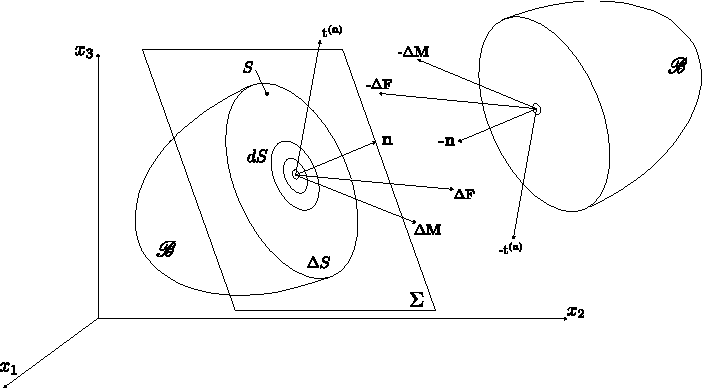
\includegraphics[width=0.75\textwidth]{images/cauchy.pdf}
\caption{Illustration of Cauchy's stress theorem. A smooth internal surface $\Sigma$ is introduced through a point $P$ of the body $\mathscr{B}$ in its current configuration. The surface divides the body into two parts, allowing the definition of internal forces $\Delta \mathbf{f}$ and moments $\Delta \mathbf{m}$ exerted across the interface. According to Cauchy's postulate, the traction vector $\mathbf{t}^{(\mathbf{n})}$ acting on the surface element $\Delta S$ depends purely on the orientation of its unit normal vector $\mathbf{n}$ at $P$. Vectors on opposing sides of the body are shown with opposite signs to represent the balance of internal forces and moments, consistent with Cauchy's stress theorem and Newton's third law.} 
\label{fig:cauchy}
\end{figure}

This traction vector $\mathbf{t}^{(\mathbf{n})}$ depends on both the spatial position and the orientation of the surface. According to Cauchy's postulate, the traction vector is the same for all surfaces through $P$ that share the same normal vector $\mathbf{n}$. Therefore, it can be written as a linear mapping from the space of normal vectors to force vectors.

Provided that $\mathbf{t}$ is a continuous function of position $\mathbf{x}$, the mapping $\mathbf{n} \mapsto \mathbf{t}$ must be linear, and so we define the Cauchy stress tensor $\boldsymbol{\sigma}$ such that:
\begin{equation}
\mathbf{t}^{(\mathbf{n})} = \boldsymbol{\sigma} \cdot \mathbf{n}, \qquad t_j^n = \sum_i \sigma_{ij}n_i.
\end{equation}
This tensor $\boldsymbol{\sigma}$ characterizes the internal force distribution at a point in the current configuration of the body.

Depending on the orientation of the surface, the traction vector $\mathbf{t}^{(\mathbf{n})}$ may not be perpendicular to the plane on which it acts, as shown in Figure~\ref{cauchydecomp}. 
Therefore, it can be decomposed into a normal component and a tangential component, defined respectively as
\begin{equation}
\sigma_n = \lim_{\Delta S \to 0} \frac{\Delta F_n}{\Delta S} = \frac{\mathrm{d}F_n}{\mathrm{d}S}
\end{equation}
\begin{equation}
\tau_n = \lim_{\Delta S \to 0} \frac{\Delta F_s}{\Delta S} = \frac{\mathrm{d}F_s}{\mathrm{d}S},
\end{equation}
where $\mathrm{d}F_n$ is the component of force normal to the surface and $\mathrm{d}F_s$ is the component of force tangential to the surface.

\begin{figure}[H]
\centering
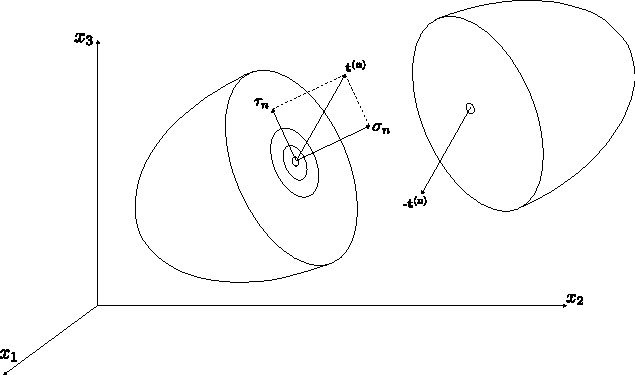
\includegraphics[width=0.75\textwidth]{images/cauchydecomp.pdf}
\caption{Decomposition of the traction vector $\mathbf{t}^{(\mathbf{n})}$ acting on an internal surface of orientation $\mathbf{n}$ into its normal and tangential components. The traction vector does not generally align with the normal vector and can be split into a normal stress $\sigma_n$, acting perpendicular to the surface, and a shear stress $\tau_n$, acting tangentially. }
\label{cauchydecomp}
\end{figure}

By definition, the Cauchy stress is defined on the current configuration. However, the deformation gradient and strain tensors are described by relating the motion to the reference configuration. Thus, not all tensors describing the state of the material are in either the reference or current configuration~\cite{bonet1997nonlinear}. Describing the stress, strain and deformation either in the reference or current configuration would make it easier to define constitutive models. To bypass this limitation, one can construct equivalent quantities to express the stress relative to the reference configuration. These are known as the first and second Piola–Kirchhoff stresses. 
The first Piola–Kirchhoff stress tensor, denoted by $\mathbf{P}$, satisfies $\frac{d\mathbf{f}}{dA}=\mathbf{PN}$ for all surfaces passing through the point on the reference configuration with normal $\mathbf{N}$ and surface area $dA$. Since $\mathbf{N}$ and $dA$ are often more easily measured at the beginning of experiments, this form of stress can be more practical. $\mathbf{P}$ can be defined as
\begin{equation}
\mathbf{P}=J\boldsymbol{\sigma}\mathbf{F}^{-T}.
\end{equation}
Because the first Piola–Kirchhoff $\mathbf{P}$ stress tensor relates forces in the current configuration with areas in the reference configuration, relating different coordinate systems, it is not symmetric. Alternatively, the second Piola–Kirchhoff stress tensor, $\mathbf{S}$, relates forces in the reference configuration to areas in the reference configuration. Therefore,
\begin{equation}
\mathbf{S}=J\mathbf{F}^{-1}\boldsymbol{\sigma}\mathbf{F}^{-T}
\end{equation}
is a symmetric tensor. Since the relations are defined within the same configuration ($d\Omega_0$), $\mathbf{S}$ is a convenient quantity for constitutive modelling.

\subsubsection{Conservation Laws}

To complete the mechanical description of deformable solids such as cardiac tissue, it is necessary to impose the physical conservation laws of mass and momentum~\cite{quarteroni2019,holzapfel2002nonlinear,chapelle2010poroelastic}. The conservation of mass states that the mass of a body in a closed system can only be created or destroyed by a known source, which means we can assume that the material density is preserved as the myocardium deforms. It is written in the reference configuration as
\begin{equation}
\frac{D\rho J}{Dt}=\hat{\rho}J,
\end{equation}
which states that the rate of change in mass, $\rho J$, is equal to the rate of mass being generated by a source $\hat{\rho}$. Here, $\frac{D}{Dt} = \frac{\partial}{\partial t} + \mathbf{v} \cdot \nabla$ defines the Lagrangian time derivative. For incompressible materials with constant density and no source of growth, the remaining mass balance equation is equivalent to $J - 1 = 0, \forall \mathbf{X} \in \Omega_0$.

Under the conditions of negligible acceleration and no body forces, the conservation of linear momentum simplifies to the null divergence of the first Piola–Kirchhoff stress tensor $\mathbf{P}$:
\begin{equation}
\text{Div} \mathbf{P} = \mathbf{0}, \quad \forall \mathbf{X} \in \Omega_0.
\end{equation}
This condition removes any dependency from the current configuration by forcing mechanical equilibrium in the reference configuration, and forms the foundation of the finite element formulation adopted in this work.

Finally, for completeness, the conservation of angular momentum states that the angular momentum of an isolated body remains constant in the absence of external forces. This translates to the requirement that the Cauchy stress tensor $\boldsymbol{\sigma}$ must remain symmetric under equilibrium conditions. In the current work, this is naturally satisfied through the use of the symmetric Cauchy stress tensor $\boldsymbol{\sigma}$.

\bibliographystyle{ieeetr}
\bibliography{../references}


\end{document}